\documentclass{article}
\usepackage[utf8]{inputenc}
\usepackage{graphicx}
\graphicspath{ {images/}}
\usepackage{wrapfig}
\usepackage{amsthm}
\usepackage{amssymb}
\usepackage{amsfonts}
\usepackage{color}
\usepackage{colortbl}
\usepackage{fancyvrb}



\title{TP4}
\author{RAJA GANAPATHY Srinivas ENGUIX Précillia}


\begin{document}
\maketitle


\section{Les nombres premiers}
$$ $$
En Python, le quotient et le reste de la division euclidienne d'un entier par un entier s'obtient de la façon suivante: pour le quotient on utilise a/b et pour le reste on cherche son modulo.
Un nombre premier est un entier naturel qui admet exactement deux diviseurs distincts entiers et positifs (qui sont alors 1 et lui-même). Ainsi, 1 n'est pas premier car il n'a qu'un seul diviseur entier positif et 0 non plus car il est divisible par tous les entiers positifs.
\newline
Parmi les nombres suivants : 1001, 2017, 3001, 49999, 89999, les nombres qui sont premiers sont les suivants : 2017, 3001, 49999. 
\newline
Nous avons écrit une fonction is prime qui prend en argument un entier n et qui renvoie true si n est premier et false si n n'est pas premier.
Les nombre de Fermat $F_0,F_1,F_2,F_3,F_4$ sont premiers mais $F_5$ n'est pas premier. 
$$ $$
     
\section{Crible d'Erasthotène, distribution des nombres premiers}
$$ $$

Nous avons calculé à l'aide du crible d'Erasthostène, la liste de tous les nombres premiers inférieurs à 200. Voici le tableau représentant :

\input{"table.txt"}
\newline
\newline
\newline

L'algorithme procède par élimination : il s'agit de supprimer d'une table des entiers de 2 à 200 tous les multiples d'un entier. En supprimant tous les multiples, à la fin il ne restera que les entiers qui ne sont multiples d'aucun entier, et qui sont donc les nombres premiers. On commence par rayer les multiples de 2, puis à chaque fois on raye les multiples du plus petit entier restant. À la fin du processus, tous les entiers qui n'ont pas été rayés sont les nombres premiers inférieurs à 200.
\newline
\newline

Suite à ça, on a écrit une fonction python primes qui prend en argument un entier n et qui renvoie la liste de tous les nombres premiers inférieurs à n. Puis on a utilisé cette fonction pour calculer la liste de tous les nombres premiers inférieurs à 1000, on a écrit cette liste dans un fichier primes.txt. La liste sera affichée dans le terminal et dans le fichier texte (10 nombres par ligne).
\newline
\newline

On note $\pi$(n) le nombre d'entiers premiers inférieurs à n, puis on a représenté graphiquement $\pi$(n) en fonction de n pour n variant de 2 à 1000. Sur le même graphique, on a rajouté la fonction n / log(n). Voici le graphique ci-dessous :
\newline
\newline
\begin{wrapfigure}{l}{1\textwidth}
        \centering
        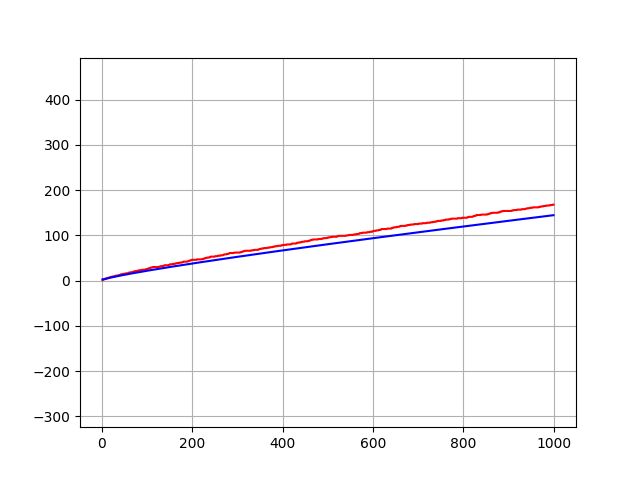
\includegraphics[width=1\textwidth]{graph2.png}
\end{wrapfigure}

$$ $$
$$ $$
$$ $$
$$ $$
$$ $$
$$ $$
$$ $$
$$ $$
$$ $$
$$ $$
$$ $$
$$ $$
$$ $$

Pour pouvoir interpréter le graphique, nous devons s'aider du théorème des nombres premiers, le voici :

\begin{wrapfigure}{l}{1\textwidth}
        \centering
        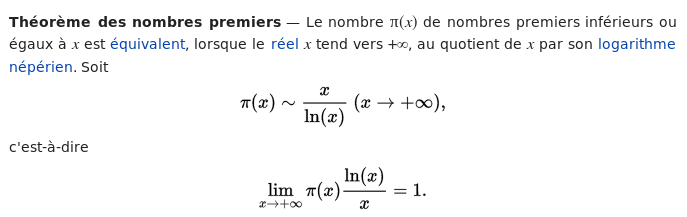
\includegraphics[width=1\textwidth]{theor.png}
\end{wrapfigure}

$$ $$
$$ $$
$$ $$
$$ $$
$$ $$
$$ $$

Donc d'après le théorème des nombres premiers et du graphique, on peut dire que $\pi$(n) et la fonction n / log n, sont équivalents.
\newline
\newline

Nous avons ensuite crée en python la table donnée dans l'énoncé, nous l'avons remplie et écrit dans un fichier texte, la voici ci-dessous :
\VerbatimInput{table1.txt}
$$ $$

\section{Factorisation d'un entier en premiers}
$$ $$

En mathématiques, et en particulier en arithmétique élémentaire, le théorème fondamental de l'arithmétique ou théorème de décomposition en produit de facteurs premiers s'énonce ainsi : tout entier strictement positif peut être écrit comme un produit de nombres premiers d'une unique façon, à l'ordre près des facteurs.
\newline
Un nombre composé est un entier naturel différent de 0 qui possède un diviseur positif autre que 1 ou lui-même. La décomposition en facteurs premiers de 924 est 2**2 x 3 x 7 x 11.
\newline
Suite à ces recherches, nous avons écrit une fonction python factors qui prend en argument un entier n et qui renvoie la liste, dans l'ordre croissante, des facteurs premiers de n, chaque facteur étant répété autant de fois que nécessaire. Ainsi, nous avons fait le test pour n = 60, n = 80 et n = 30.
$$ $$

\section{PGCD de deux entiers, identité de Bézout, algorithme d'Euclide}
$$ $$

En arithmétique élémentaire, le plus grand commun diviseur ou pgcd de deux nombres entiers non nuls est le plus grand entier qui les divise simultanément.
Pour calculer le pgcd, nous sélectionnons les facteurs communs, ensuite nous effectuons le produit. Ici, 4864 = 2**8 x 19 et 3458 = 2 x 7 x 13 x 19 donc pgcd(4864, 3458) = 38.
$$ $$
Voici l'identité de Bézout :

\begin{wrapfigure}{l}{1\textwidth}
        \centering
        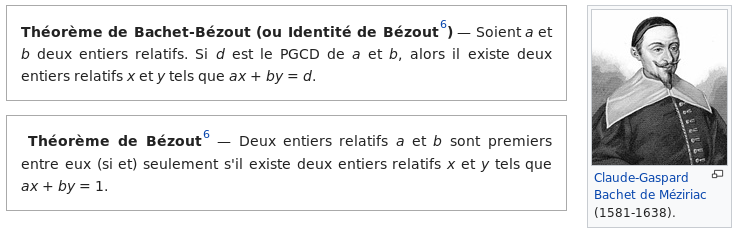
\includegraphics[width=1\textwidth]{bezout.png}
\end{wrapfigure}

$$ $$
$$ $$
$$ $$
$$ $$
$$ $$
$$ $$ 

L’algorithme d’Euclide permet de calculer le pgcd de deux entiers naturels non nuls a et b. On procède de la manière suivante : On effectue la division euclidienne de a par b. On note r le reste (on n’utilise pas le quotient). On remplace ensuite a par b et b par r. Tant que le reste est différent de 0, on réitère le procédé. Après un certain nombre d’itérations, on obtiendra un reste égal à 0. Le pgcd de a et de b est alors le reste précédent (c’est à dire le dernier reste non nul). 
\newline
\newline
A l'aide de l'algorithme d'Euclide étendu, le pgcd des 2 nombres a = 4864 et b = 3458 est 34. Pour obtenir les coefficients de Bézout, il suffit de remonter l'algorithme d'Euclide à l'envers, on trouve alors les coefficients de Bézout : x = 32 et y = -45. 
\newline
\newline
Nous avons écrit une fonction python euclide qui prend en arguments 2 entiers a et b, qui renvoie x, y, d, où d est le pgcd de a, b et x, y les coefficients de Bézout. On obtient d = 38, u = 32, et v = -45.
$$ $$

\section{Chiffrement RSA}
$$ $$

Le chiffrement RSA est un algorithme de cryptographie asymétrique, très utilisé dans le commerce électronique, et plus généralement pour échanger des données confidentielles sur Internet.
\newline
\newline

Nous n'avons pas eu le temps de poursuivre le reste de la partie RSA, car nous devions commencer le projet pour le partiel.

$$ $$

\section{Analyse de la séance de TP}

$$ $$

Le début du TP a été assez simple, nous avons manqué de temps pour la partie chiffrement RSA. Dommage, car c'était le TP le plus intéressant. Nous remarquons une forte évolution au niveau du codage python ainsi que du latex.
\newline
C'est une matière très intéressant avec beaucoup de ressource. 








\end{document}


